\documentclass[11.5pt]{sig-alternate}
\usepackage[defaultlines=3,all]{nowidow}
\usepackage{hyperref}
\usepackage{tabularx}
\usepackage{graphicx}
\usepackage{blindtext}
\usepackage[utf8]{inputenc}
\usepackage[english]{babel}
\usepackage{csquotes}
\usepackage{lastpage}
\usepackage{comment}
\usepackage{dirtytalk}
\usepackage{xcolor}
\usepackage{hanging}
\usepackage{wrapfig}
\usepackage[backend=biber, style=apa]{biblatex}
\addbibresource{notation.bib}
\usepackage{authblk}
\usepackage{caption}
\usepackage{graphicx,subfigure}
\usepackage[normalem]{ulem}
\useunder{\uline}{\ul}{}
\usepackage{authblk}
\usepackage{enumitem}
\usepackage[utf8]{inputenc}
\usepackage{cuted}
\usepackage{fancyhdr}
\pagestyle{fancy}
\usepackage{lipsum}
\usepackage{amsmath}
\usepackage{stix}
\usepackage{booktabs}
\usepackage{ragged2e}
\usepackage{xurl}
\usepackage{tabularray}
\usepackage{float}
\usepackage{array}
\usepackage{microtype}
\DeclareUnicodeCharacter{0360}{\eth}
\renewcommand{\headrulewidth}{0pt}
\renewcommand{\footrulewidth}{0pt}
\setlength\headheight{80.0pt}
\addtolength{\textheight}{-80.0pt}
\chead{%
  \ifcase\value{page}
  % empty test for page = 0
  \or 
\includegraphics[width=\textwidth]{headerimage.png}% page = 1
 \or 
\includegraphics[width=\textwidth]{headerimage.png}% page = 2
  \or 
\includegraphics[width=\textwidth]{headerimage.png}% page = 3
  \or 
\includegraphics[width=\textwidth]{headerimage.png}% page = 4
 \or 
\includegraphics[width=\textwidth]{headerimage.png}% page = 5
  \else
  
\includegraphics[width=\textwidth]{headerimage.png}
  \fi
}
\newcommand{\nextitem}{~~\llap{\textbullet}~~}
%\chead{
\includegraphics[width=\textwidth]{headerimage.png}}
\hypersetup{
    colorlinks=true,
    urlcolor=blue
}
\captionsetup[figure]{font = it,}
\captionsetup[table]{font = it,}
\let\oldabstract\abstract
\let\oldendabstract\endabstract
\makeatletter
\renewenvironment{abstract}
{\renewenvironment{quotation}%
               {\list{}{\addtolength{\leftmargin}{1em} % change this value to add or remove length to the the default
                        \listparindent 1.5em%
                        \itemindent    \listparindent%
                        \rightmargin   \leftmargin%
                        \parsep        \z@ \@plus\p@}%
                \item\relax}%
               {\endlist}%
\oldabstract}
{\oldendabstract}
\makeatother

% Left align captions
\captionsetup{justification   = raggedright,
              singlelinecheck = false}


\begin{document}

\title{Engaging Students with Disabilities in Universally\\
Designed Science Education}

\author[1]{\large \color{blue}Latifa Sebti}
\author[1]{\large \color{blue}Michelle L. Damiani}
\affil[1]{Rowan University}

\toappear{}
%% ABSTRACT
\maketitle
\begin{@twocolumnfalse} 
\begin{abstract}
\item 
 \textit {Increased student diversity in classrooms and the need for equitable STEM
opportunities for all, creates an impetus for educators to establish inclusive and equitable
environments and use teaching practices that facilitate meaningful learning for all students in
science education. This article offers a three-part framework for combining inclusive philosophy,
the science and engineering practices, and Universal Design for Learning (UDL). The article
is intended to help teachers and teacher educators universally design science education to
level the science learning field through access and equity for all students, including students
with disabilities. We advocate for the use of four practices: creating an inclusive community of
science learners, planning for big ideas over time, engaging students in sense-making through
model-based inquiry, and engaging students in cooperative learning and science talk. Science
teachers can use these practices to universally design science education and enhance science
learning and STEM interest for underrepresented students. In the article, we provide visuals
and tools for teachers to support implementation of the universally designed science practices.}
     \\
     \\
     Keywords: Students with disabilities, engagement, inclusive science education, Universal
Design for Learning, model-based inquiry, science access and equity, Next Generation Science
Standards.
\end{abstract}
\end{@twocolumnfalse}




%% AUTHOR INFORMATION


\textbf{*Corresponding Author, Latifa Sebti}\\
\href{mailto: sebtil45@rowan.edu }{(sebtil45@rowan.edu)} \\
\textit{Submitted January 6, 2021 }\\
\textit{Accepted May 20, 2021} \\
\textit{Published online November 22, 2021} \\
\textit{DOI:10.14448/jsesd.13.0013} \\
\pagebreak
\pagebreak

\vspace{5mm}
\section*{\vspace{140mm}}
\begin{large}
\section*{ENGAGING STUDENTS WITH DISABILITIES IN UNIVERSALLY DESIGNED SCIENCE EDUCATION}

Consider the following vignette.\textit{ Mrs. Robinson is a new teacher in a diverse middle school. She was assigned an inclusive science class that includes students with various cultural backgrounds, socioeconomic and disability status. She has four students with Individualized Education Programs (IEPs) including one student with an autism label, one student with an intellectual disability label, and two students with learning disability labels (dyslexia and dyscalculia), as well as two students with 504 plans for untimed tests. She was struggling to meet everyone’s needs and began thinking about equitable and accessible practices to meaningfully integrate and engage all students in her classroom.}

Mrs. Robinson’s question is common among teachers: How do I meet the standards and meet the needs of all of my students? Every teacher must be prepared to address the increasing diversity of learners in their classrooms and content areas (National Center for Education Statistics, 2019). The inequity in learning outcomes between students with and without identified disabilities places a high priority on best instructional practices that facilitate meaningful access for all students in science education. We advocate beginning with an ideological foundation that presumes student competence (Jorgensen, 2005). The lack of effective instruction and lowered academic expectations both lead to poor science learning outcomes for students with disabilities (Horowitz, et al., 2017). Meanwhile, positive classroom climates and inclusive and equitable teaching practices positively correlate with enhanced students’ performance and engagement in STEM careers (C-abrera et al., 2001). Inclusive pedagogies such as student-centered approaches, inquiry-based instruction (Windschitl \& Barton, \\2016), and UDL (Meyer, et al., 2014) can be used to design inclusive classroom environments and instruction and work to address the opportunity gap (Ladson-Billings, 2013). 

In this article, we hope to help teachers and teacher educators do the following: 
\begin{enumerate}[label=\alph*]
 \item Develop awareness of the alignment of inclusive and UDL practices with the Next Generation Science Standards (NGSS Lead States, 2013); 
    \item Learn about research-based and universally designed science classroom practices and tools that improve engagement, academic, and social performance for students with disabilities.
    \item Understand steps for how to implement universally designed science practices to improve curriculum accessibility for diverse learners. 
\end{enumerate}

\section*{A CONCEPTUAL FRAMEWORK FOR UNIVERSALLY DESIGNED INCLUSIVE SCIENCE EDUCATION}

In this section, we outline a conceptual framework that includes three components for universally designing science education with three guiding questions. The components with their guiding questions represented in Figure 1 include: 1. Inclusive philosophy (what teachers believe); 2. Science and engineering practices (what teachers teach); and 3. Universal Design for Learning (how teachers do it). We argue that in order to achieve a more cohesive practice of universally designed science education, these components must be used in combination, and science teachers must have a good working understanding about how each component contributes to the overall goal of supporting all students with science learning. From there, teachers can use these components to make informed pedagogical decisions about how to best deliver science specific content and meet the needs of all of their students.

\begin{figure}[t]
    \centering
    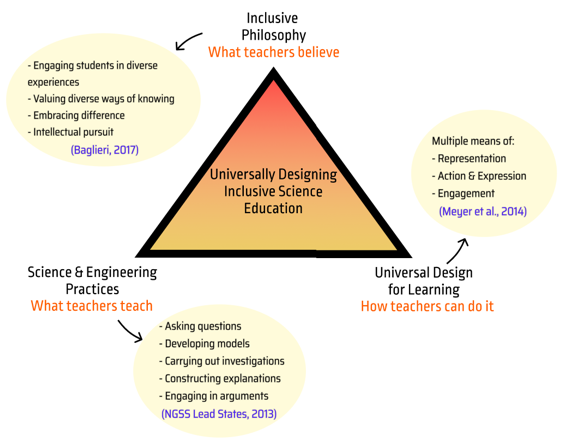
\includegraphics[width=1\linewidth]{fig1.png}
    \caption{Universally Designed Inclusive Science Education Framework}
\end{figure}

Science education has long framed learning “as engagement with scientific practices” (Brickhouse et al., 2000, p.441). Literature also indicates that some students with disabilities experience science learning as inaccessible with one reason being the extensive amount of academic language involved in science lessons and the inductive and deductive thinking required for scientific reasoning (Mastro-pieri et al., 2006). Science learning also requires students to make sense of observable phenomena, abstract concepts, and complex science practices including controlled experimentation, data collection, and data analysis (Puttick \& Mutch-Jones, 2015). The perceived difficulty of science subject matter has contributed to limiting access to the general education science curriculum for many students with disabilities. Consequently, students with disabilities are underrepresented in STEM fields due to the lack of meaningful independent experience, low expectations, and limited educational opportunities (Dunn et al., 2012). Furthermore, classroom community and the design of the learning environment are key factors in shaping students’ science identities and supporting the shift from a sense that "science is not for me” to a sense of science expert (Windschitl \& Barton, 2016, p. 1119). Known exclusions from the science curriculum, and within the discipline more broadly, underscore the need for more flexible, inclusive, and student-centered approaches to science teaching. 

Windschitl and Barton (2016) discuss this instructional gap as follows:

\begin{quotation}
    The aspects of instruction known to support engagement and learning— such as maintaining an environment of high expectations, responding to student thinking, and linking activity with science ideas and with the out-of-school experiences of young learners—are precisely where classroom teaching appears weakest (p. 1102).
\end{quotation}

Additionally, Universal Design for Learning resea-rch supports that learners need to be actively engaged in learning experiences and provided opportunities for choice in educational activities (Meyer et al., 2014). The multiple means of engagement principle of UDL aims to tap into students’ interests, challenge them, and motivate them to learn (CAST, 2018). Thus, the UDL framework is well aligned to calls for improving science teaching as identified by the science education field. Following is a detailed discussion about each of the specific components of our proposed framework supported by relevant literature and contextualized with growing examples explained through vignettes. 

\subsection*{Component 1: Inclusive Philosophy (What Teachers Believe)}

\textit{Elijah Ditchendorf was a student transitioning from elementary to middle school who self-ide-ntified as dyslexic, had an IEP, and was an active member of his IEP planning team. Ditchendorf and his family were told by his sixth grade science teacher that he could not be recommended for accelerated science in middle school because “I had reached his full potential. Midway through seventh grade, my accelerated ma-th teacher said, ‘Why aren’t you in accelerated science?’ I said, they didn’t think I was smart enough.” (National Center for Learning Disabilities, 2017, n.p.). Mrs. Robinson’s proactive effort to meet the needs of all of her students may prevent a student like Elijah from being excluded.}

Elijah's story demonstrates the critical importance of understanding disability beyond educational labels and deficit-driven perspectives that may justify limiting students' learning opportunities in sc-hool. Disability studies in education (DSE) offers educators an opportunity to expand their goals as inclusive educators by intentionally disrupting inequities. For teachers this could include, presuming competence, maintaining high expectations, a-nd ensuring access to and engagement with rigorous academics. Koomen and colleagues (2018) urge listening to the voices of students as experts of inclusion “who tell us in their own words what practices really work best for them in an inclusive classroom” (p. 363). Centering disabled voices and students' experiences is also a specific aim of the field of disability studies and is an integral part of changing perceptions of disability in education by honoring individuals with disabilities as the authorities of their own lived experiences (Ferguson \& Nusbaum, 2012). The impact of teachers' perceptions of disability is illustrated by the disparate outcomes that came because of the different beliefs held by Elijah’s sixth and seventh grade science teachers.
	
 We start our discussion about inclusive philosophy by first recognizing the legal underpinning for inclusive education for students in U.S. schools. The Individuals with Disabilities Education Act (1997) mandated that students with disabilities receive a “free appropriate public education” in the "least restrictive environment." According to the law, students with disabilities must be provided with supplemental aids and services to support an appropriate education, with the expectation that students who receive special education services are included in the general education classroom as often as possible. Furthermore, the Supreme Court’s ruling in the Endrew Decision created a higher substantive standard for determining ‘meaningful educational benefit’ with an expectation that most students will be fully integrated and make meaningful progress in the general education curriculum, and that progress will be reflected in the student’s IEP (Endrew F. v. Douglas County School District, 2017). We recognize inclusive education as a student right and the responsibility of all teachers.
	
 Practices of inclusive education intentionally \\grounded in DSE and aligned with critical pedagogy, multiculturalism, and social justice in schools, can create welcoming general education classrooms responsive to disability and difference (Baglieri, 2017). To achieve the aims of inclusive education, we need to address how students are excluded from the science curriculum. As a starting point, DSE shifts conceptualizations about students such that "students with diverse learning needs are not the problem; barriers in the curriculum itself are the root of the difficulty" (Hitchcock, et al., 2002, p.9).

Practitioners need to understand meaningful inclusion in order to avoid the risk of exclusion even when students with disabilities are physically present in classrooms. As Ferri (2006) stated, “students can be physically included but not conceptually included in the mind of the teacher” (p. 292). Meaningful inclusion responds to students’ individual needs and interests through a true sense of belonging in a supportive community, rather than positioning students’ needs as a burden. With this understanding, we can move beyond promoting one way of teaching based on the “myth of the normal child” (Baglieri et al., 2011, p. 2124). In inclusive education, students with disabilities and neurodiverse students (Armstrong, 2018) should not be expected to learn the same thing, in the same way, at the same pace, and produce the same product, but instead be provided flexible engagement and assessment opportunities.

For any inclusive educator, practicing meaningful inclusion and developing an inclusive classroom community involves both an ideological commitment to support students with disabilities and the implementation of research-based practices (Ferguson \& Nusbaum, 2012). Presuming students competence and using stren-gths-based approaches are foundational to the rigorous work needed around achieving equity in science education and accepting diversity as a norm rather than an exception (Tsu et al., 2014). Strengths-based IEPs should be implemented with the purpose of sustaining high expectations and encouraging students to reach hi-gher levels of academic achievement through str-engths-based services, supports, and goals (Elder et al., 2018). The design of learning experiences should honor students’ sense-making repertoires \\with various ways of reasoning and communicating as well as value and respond to their voices, experiences, funds of knowledge, and perspectives (Gay \& Kirkland, 2003). It is essential "to ensure that individual differences do not mitigate access and engagement" (Edyburn, 2010, p.36). Therefore, science teaching strategies must be designed to improve curriculum accessibility and engagement for all students, and improve learning outcomes inclusive of, and with the attention to the value that students’ diverse experiences, abilities, language, and cultural backgrounds bring to the science classroom. 

\subsection*{Component 2: Science and Engineering Practices (What Teachers Teach)}

\textit{Mrs. Robinson is thinking about her science units and how to link them to topics that are interesting to her students to enhance their engagement. She asks herself about the important observable and relevant phenomena that students should understand and how they can represent a model that could help them make sense of the unit’s big ideas. For example, in the sound energy unit, she could use a video of a singer whose voice makes a glass break as an anchoring event to get her students thinking about the cause of this phenomenon, the concept of sound as energy, the characteristics of sound waves, and resonance. Then her students will construct an explanatory model and argue from evidence to show the concepts and conditions involved.}
	
 The science and engineering practices draw from reform-based science teaching that employs st-udent-centered inquiry. The science standards encompass both the framework for science education (National Research Council, 2012) and the NGSS (2013) with its three dimensions: science and engineering practices, crosscutting concepts of science, and disciplinary core ideas. These dimensions aim to help students improve their understanding and use of scientific knowledge, ideas, and inquiry processes and their application in real-world situations. According to Ambitious Science Teaching, (Windschitl et al., 2018) science education is guided by four core practices: (a) planning for engagement with big science ideas, (b) eliciting students’ ideas, (c) supporting ongoing changes in thinking, and (d) drawing together evidence-based explanations. Educational research has demonstrated the effectiveness of an inquiry-based approach providing opportunities for hands-on learning and group interaction that can create high interest and alternative ways for students with disabilities to understand the real world (Mastropieri \& Scruggs, 2005).
	
 Teaching aligned to the NGSS (2013) requires a shift away from presenting information for memorization to supporting students’ explorat-ions of phenomena through the process of building models, providing explanations, and using evidence to support their thinking (Krajcik \& Mun, 2014). Concerningly, there is a tendency to accommodate students with disabilities by relying on teachers and peers to accomplish hig-her order thinking activities. This occurs when teachers assume that students are unable to meet rigorous standards and engage in inquiry, rather than developing supports that encourage autonomy, as the major adaptation (Kahn, et al., 2017). The goal of inclusive science instruction is not to make science content easier by watering it down, but rather as Ellis (1997) argues by actively “watering up” the curriculum so that all students have opportunities for deep learning and thinking. There are various effective, research-based instructional models readily available within science teaching that are grounded in active participation and that can empower students toward equitable performance outcomes These models include the inquiry continuum: confirmation inquiry, structured inquiry, guided inquiry, and open inquiry \\(Banchi \& Bell, 2008) and the 5E model: engage, explore, explain, elaborate, and evaluate (Bybee, et al., 2006). Guided-inquiry approaches are demonstrated to have effective outcomes for students with disabilities (Aydeniz et al., 2012). 
	
 The NGSS (2013) aim to engage all students in conceptual thinking by “doing science” involving the content and the process of science learning (Kang \& Zinger, 2019; Penuel \& Reiser, 2018). The NGSS (2013) demonstrate a comprehensive vision of inclusive science for underrepresented groups, including students with disabilities and preparing all students for STEM-related college studies or careers. Appendix D in NGSS (2013) presents effective classroom strategies with diverse student groups capitalizing on their cultures as valuable resources and connecting their background knowledge with science learning (Januszyk et al., 2016). Such strategies help “students of all backgrounds to deeply understand fundamental science ideas, participate in the practices of science, solve authentic problems together, and learn how to continue learning on their own” (Windschitl et al., 2018, p. 3). All of these expected outcomes can support an inclusive universally designed approach to science learning.

\subsection*{Component 3: Universal Design for Learning (How Teachers Can Do It) }

\textit{To proactively design UDL-aligned lessons, Mrs. Robinson should first know her students including their interests, strengths, needs, talents, lived experiences, and the community and cultural knowledge that they bring to the classroom. Next, she needs to pinpoint barriers in the curriculum that impede engagement and progress for any student and plan for ways to make the goals, materials, instructional methods, and assessments inclusive through flexible, accessible, and engaging learning experiences. For example, Mrs. Robinson plan-ned for multiple means of representation by building in the option for all students to access scientific information thr-ough digital text. The opportunity for visual access and text-to-speech conversion met her students' stated needs in the areas of reading decoding and reading comprehension, but also potentially created access points that benefit other students as well. For example, English language learners may benefit from the language tools afforded by the use of digital texts, and/or students for whom listening comprehension is a strength could have the option to increase the audio reading speed. Mrs. Robinson has also planned to help all students access content from textbooks or lectures by activating prior knowledge through questions and scaffolds, providing multiple examples, highlighting important information, and offering adjustable levels of challenge using flexible groupings.}

Universal Design for Learning was developed by the Center for Applied Special Technology (CAST) in the early 1990s as a research-based framework based on neuroscience and cognitive-social learning. It evolved into an educational model that consists of designing educational go-als, methods, materials, and assessments to improve accessibility. Like science education, UDL (Meyer et al., 2014) recognizes the need for student engagement in purposefully varied ways with attention to eliminating access barriers fr-om the outset. The UDL framework is organized around three principles: 1. Multiple mea-ns of representation; 2. Multiple means of action and expression; and 3. Multiple means of engagement. These principles are also often discussed as the “what” of learning, the “how” of learning, and the “why” of learning respectively. In brief, the three principles involve providing information in multi-modal ways (representation); providing students with options to participate in learning activities and demonstrate what they have learned (action and expression); and motivating students through choice, experience, and real-life application (engagement). 

All of the principles are organized through checkpoints designed for students to access learning, build skills, and internalize strategies toward developing learners who are resourceful and knowledgeable, strategic and goal-oriented, and purposeful and motivated (CAST, 2018). “Universal Design for Learning focuses on building supports proactively into lesson goals, curriculum resources, instructional practices, and assessments” (Ok et al., 2016, p. 1). However, before designing lessons or learning activities, it is first necessary to know your students by assessing their prior knowledge, interests, and needs. This critical first step allows teachers to plan purposefully for their students. The next step is to identify any known or potential barriers to learning for all students. At this point, a teacher is ready to consider how they will teach specific science skills or concepts using flexible goals, materials, methods, and assessments for students (see Figure 2).

\begin{figure}[t]
    \centering
    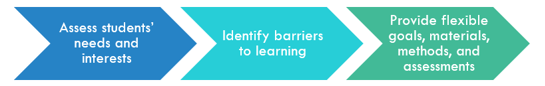
\includegraphics[width=1\linewidth]{fig2.png}
    \caption{Steps for Designing UDL-aligned Lessons}
\end{figure}

This framework is similar to differentiated instruction that also uses these three planning steps for individual students or groups of students across the areas of content, process, product, and learning environment (Tomlinson, 2001). However, in UDL the focus shifts away from individual students or groups of students to the design of the learning environment and instruction by proactively removing any barriers. This framework shapes equitable attitudes and practices for all students, rather than focusing on students with identified disabilities. Watt and colleagues (2013) identify how UDL and science education are well aligned stating that, “as part of UDL, providing a range of supports and a systematic way for students to organize and make connections, even within an inquiry-based classroom is a perfect marriage for success of students with a range of needs” (p. 41). Thus, a range of supports for students should draw on research-based and evidence-based practices including universally designed tools and assistive technologies. Research shows that educational “technology holds significant promise for improving scientific learning opportunities for students with disabilities” (Marino, 2010, p.6). Many technologies such as touch screens, voice dictation, text to speech, captioning, and word prediction began as ways to assist students with disabilities, but can be beneficial to all students. Digital science teaching tools, such as the ones we present in Table 2 below, are another form of assistive technologies that can offer flexibility, access, and communication options for the science classroom. 

Now that we have explained each component of the three-part framework in detail, the remainder of this article discusses ways for teachers to apply these practices.

\section*{IMPLEMENTING UNIVERSALLY DESIGNED INCLUSIVE SCIENCE EDUCATION: ENGAGEMENT IN ACTION}

\textit{Mrs. Robinson has identified her students’ learning needs, strengths, and interests and understands the components of the conceptual framework presented above. She is willing to implement these practices in her classroom, but needs direction on connecting theory to practice. The practical steps in this next section would help Mrs. Robinson engage students with disabilities in universally designed science education. }

We have identified four interconnected practices situated within the three-part framework while keeping in mind the larger goals of achieving equity and access for all students in science education (see Figure 3). Throughout this section, the tables serve as visual tools to help teachers make explicit connections to their own practice. We encourage teachers to use these tools and expand their implementation as they see most useful in their classroom context. Engaging students in universally designed science learning and science doing translates into giving students opportunities to participate in an inclusive science classroom community, connect their knowledge to big ideas, get involved in sense-making activities through experiential mo-del-based learning, and engage in cooperative learning with science talk. 

\begin{figure}[t]
    \centering
    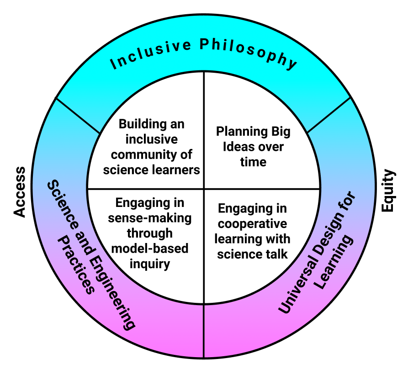
\includegraphics[width=1\linewidth]{fig3.png}
    \caption{Engaging students in Universally Designed Inclusive Science Education}
\end{figure}

\subsection*{Practice 1: Creating an Inclusive Community of Science Learners}

\textit{As a teacher committed to creating equitable science classrooms, Mrs. Robinson seeks to build a democratic and socially just science community culture that encourages open dialogue and provides a safe environment for students to take appropriate learning risks. She realizes that her beliefs about her students will affect how she approaches teaching them. By using a strengths-based lens, she sees how all of her students are capable and will benefit from science instruction.}

Through an inclusive philosophical approach, teachers’ beliefs about students can translate to opportunities for every student to have an engaged sense of agency and to develop their identities as scientists within the classroom and in their communities. Table 1 offers five steps for how a teacher might specifically develop an inclusive science community in their practice.

\begin{table*}[t]
\caption{\textit{Building an Inclusive Science Classroom Community}}
\begin{tabular}{ll}
\hline
Steps & Description \\ \hline
Step 1 & Welcome students’ ideas, experiences, and questions with clear social and conversation norms, respect for others, and a disposition to share and revise ideas in a collaborative and safe scientific environment (Berland \& Reiser, 2011). \\ \hline
Step 2 & Presume competence for all students and value their unique identities, needs, competencies, and the knowledge they bring to the classroom (Baglieri, 2017; Windschitl et al., 2018). \\ \hline
Step 3 & Engage students in authentic and meaningful scientific inquiry experiences with a range of participation options, interactions with the teachers and peers, and opportunities to do science (Sampson et al., 2011). \\ \hline
Step 4 & Provide cooperative learning experiences and seating plans organized in a welcoming environment of acceptance and respect (Jones \& Sterling, 2011) where students have safe access to materials and experiences (Trundle, 2008). \\ \hline
Step 5 & Make diversity visible and pursue a culturally responsive approach by including the contributions of scientists from marginalized groups including people with disabilities, building on prior cultural funds of knowledge, and understanding the sense-making practices of diverse communities (National Research Council, 2012). \\ \hline
\end{tabular}
\end{table*}

Building an inclusive community of learners is part of the high leverage practice in special education for establishing a consistent, organized, and respectful learning environment (McLeskey et al., 2017). Once teachers build this foundation, then they can engage their students in meaningful science learning opportunities and connections starting with big ideas and getting to sense-making activities through cooperative learning and science talk. 

\subsection*{Practice 2: Planning for Big Ideas over Time}

\textit{Now, Mrs. Robinson identifies the science big ideas in her lesson with attention to the “what” and “why” of learning. When writing the learning objectives, she uses verbs such as “identify, determine, solve, and justify,” instead of verbs such as “read, write, or speak.” These terms focus on the skills of science thinking and make the goals accessible to diverse learners by avoiding performance criteria written around a particular way of expressing oneself that could create barriers for demonstrating understanding of the scientific concepts. To present the big ideas for her unit, Mrs. Robinson begins by striking a tuning fork and then placing it next to water causing the water to splash. The big idea is to get her students asking questions to determine that sound waves carry energy and travel through a medium.}
	
 The NGSS (2013), UDL (Meyer et al., 2014), and science education research have a shared focus on helping students build a broader, more contextualized understanding of concepts over individual facts. Big ideas are the intended goals that provide a conceptual and relational understanding of science concepts. Clearly communicating learning goals and big ideas to students encourages them to “focus, self-regulate, and monitor their levels of cognitive, emotional, and physical engagement” (Basham \& Marino, 2013, p.11). Teachers should present academic language and big ideas toward the goal of developing meaningful connections and conversations about their learning (Watt et al., 2013). In addition, teachers should explicitly teach academic language as a means to reduce barriers related to lack of background knowledge about new scientific concepts. Therefore, providing options that supply or activate prerequisite information is critical. Such options include (CAST, 2018): 

\begin{itemize}
\item   [--]Using anchor instruction (e.g., visual imagery, anchoring events);
\item   [--]Using advanced organizers (e.g., concept maps, KWL charts);
\item 	[--]Pre-teaching prerequisite concepts through models or representations;
\item 	[--]Connecting concepts with relevant meta-phors and analogies;
\item 	[--]Making interdisciplinary connections (e.g., teaching reading strategies)
\end{itemize}

Planning for engagement with big ideas involves teachers’ identification of intended science concepts, selection of an anchoring event and essential question to organize and support students’ thinking, and sequencing of ideas and activities as they seek to answer the essential questions (Windschitl et al., 2018). For this purpose, teachers can create concept maps to pinpoint the unit activities building toward the big ideas and the narrative storyline of a unit (Puttick \& Mutch-Jones, 2015). This helps students construct sophisticated ideas using evidence that builds on their prior understanding as they engage in explaining phenomena. Thinking about big ideas and making connections between practices and activities using a storyline, students can gradually develop integrated understanding to reach the level of expected proficiency and avoid compartmental understanding (Krajcik \& Mun, 2014). These big ideas need to be built over time for students to make connections to different science concepts, revise, and improve their understanding while being engaged in sense-making investigations.


\subsection*{Practice 3: Engaging in Sense-making Through Authentic Model-based Inquiry}

Using experiential model-based learning, Mrs. Robinson has a central role in facilitating her students’ three‐dimensional learning to support her students with disabilities in sense-making that pushes them to higher-level thinking. She engages her students through phenomena, such as salt and sugar dissolving in the food, phone charging using electricity, and clothes clinging on bodies. All of her students are more likely to relate to these concrete real-world events and be motivated to ask new questions that they identify as necessary to construct models and explanations of phenomena. In this way, Mrs. Robinson’s teaching allows for applied learning rather than isolated or decontextualized concept understanding.

After making big ideas clear to students and activating their prior knowledge, teachers center instruction around a phenomenon or discrepant event that sparks interest and generates curiosity and questions. Eliciting students’ initial thoughts makes their thinking visible as a formative assessment and identifying students’ misconceptions. Students can then be prompted to create scientific models to predict or explain phenomena using diagrams, drawings, physical representations, analogies, and digital simulations (Windschitl et al., 2018). The eight NGSS science and engineering practices presented in Figure 5 center around phenomena that drive science inquiry and investigation (NGSS, 2013). 
%figure 5?
\addtocounter{figure}{1}
\begin{figure}[t]
    \centering
    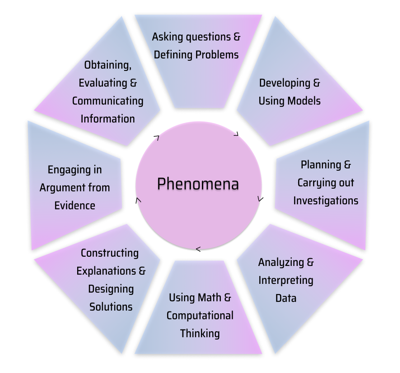
\includegraphics[width=1\linewidth]{fig4.png}
    \caption{The Eight NGSS Science and Engineering Practices}
\end{figure}

By centering on phenomena, students are more likely to be motivated to ask questions, test their ideas through investigation, and use evidence to explain science events. The results of this engaged process allow students to develop more refined and scientifically accurate understandings of the natural world. Engaging in scientific modeling also allows students to visualize abstract concepts, such as energy and force. Additional resources about model-based practices, as well as practical planning and scaffolding tools are available online through Ambitious Science Teaching (Ambitious Science Teaching Development Group, 2020). For many students with disabilities supplementing the inquiry process with specific structure, and explicit instruction and feedback may be most successful (Watt et al., 2013). Teachers should also adjust the level of challenge presented to all students without reducing challenging learning opportunities for students with disabilities. An important part of the process is building in opportunities for students to actively reflect, assess, and self-monitor their learning and engagement (Summy \& Fetters, 2018).

In order to further inclusively design students’ experiences with the science and engineering practices, teachers should address phenomena within home and community contexts, and give students opportunities to use their out of school experiences to make meaningful connections to solve issues with local relevance and real-life application. These kinds of inclusive and culturally responsive learning opportunities with science content can generate students’ interests in STEM-related college studies and careers (Jan-uszyk et al., 2016). The major goal of science education is to “provide all students with the background to systematically investigate issues related to their personal and community priorities” (National Research Council, 2012, p. 278). Activities that build on students’ interests, everyday experiences, and cultural practices (i.e., food chemistry, local climate change, local ecosystems, and physical traits in families) promote active participation and sustained learning in science classrooms.

\subsection*{Practice 4: Engaging in Cooperative Learning with Science Talk}

\textit{Mrs. Robinson has planned to use a science talk protocol to have students talk out their ideas like scientists using evidence that they have collected about animal structures and functions. She has already established group norms for participating in science talks with clear goals and rules. She reminds students of these expectations before she gives them the open-ended science question to discuss in small groups. Having students work in small heterogeneous groups gives students more engaged discussion time and allows Mrs. Robinson to meet the needs of individual students and groups based on where they are in the learning process.}

Research shows that students with disabilities greatly benefit from small-group learning through increased achievement, peer acceptance, and self-efficacy and “overcome obstacles they might not overcome working alone” (Jenkins et al. 2003, p. 280). From a universal design approach, cooperative learning strategies allow students to work together to find solutions to scientific issues to ensure active participation and engagement of all students (Scruggs et al., 2007). Students working in pairs or groups draw on their prior knowledge, allows them to debate different ideas, and encourages them to seek additional information to extend their understanding and generate solutions (Kuhn, 2015). Use of cooperative learning activities in a supportive learning environment creates conditions whereby students learn from each other and become social and academic peer support partners to reach a common learning goal (Guðjónsdóttir \& Óskarsdóttir, 2016). Thus, collaborative learning designed through inquiry-based science provides a strengths-based and student-centered way for students to make progress toward shared learning goals.

Full engagement in the science and engineering practices necessitates opportunities for student interaction and dialogue. Using science talk protocol provides a universally designed way for students to theorize together, promotes equitable conversation, and builds literacy skills. In fact, “the ultimate goal of science talk is to create a discourse-rich classroom culture where the natural synergy between language and meaning making supports all students in expressing ideas, developing language and acquiring new knowledge of scientific phenomena” (Exploratorium, 2021). The Ambitious Science Teaching Development Group (2020) offers a protocol for teachers wondering, “How do I begin to shift my classroom culture away from right answers towards collaborative knowledge construction talk?” Exchange of ideas around problem solving stimulates science talk that plays an important role in prompting and supporting students' scientific sense-making based on observations, claim, and evidence. In a safe and welcoming classroom environment, “together, strong norms, predictable routines, and strategic scaffolding enable talk to flourish” (Windschitl et al., 2018, p.65). Engaging in scientific discourse and practices of science offers a rich language-learning opportunity for students and an opportunity to leverage community discourse (National Research Council, 2012).

\subsection*{Additional Consideration: Aligning Instruction through Use of Technology}

More than ever before, digital tools are an essential part of the learning landscape. Educational technology and interactive digital tools and platforms have become even more necessary and sought after in the virtual learning environment. Many science notetaking, data/evidence recording, and visual thinking and mapping tools originally used in pencil and paper format, are now available as digital tools for the science classroom. Table 2 offers teaching ideas for using digital tools in the science classroom including interactive science notebooks, science games, and digital graphic organizers. Use of such tools fits well into universally designed inclusive strategies as they can promote deeper understanding of concepts with flexible opportunities for practice for many students. 

\begin{table*}
\caption{Examples of Universally Designed Digital Tools for Science}
\begin{tabular}{ll}
\hline
Digital Tools & Description \\ \hline
Universally designed interactive science notebooks & Using science notebooks can enhance students’ experiences as scientists and writers of scientific ideas (Collins \& Fulton, 2017). Universally designed science notebooks (UDSN) provide access to flexible tools, materials, and supports, effectively engage students and help overcome barriers in traditional notebooks related to recording, organizing, analyzing, and interpreting data (Rappolt-Schlichtmann et al., 2013). Some examples of how UDL principles are integrated into UDSN and interactive science notebooks are through built-in text-to-speech technology, English-to-Spanish translation, descriptions for images, a multimedia glossary, animated visuals, actual photographs, diagramming tools, etc. \\ \hline
Universally designed digital science games & UDL-aligned digital games can support knowledge transfer between virtual and classroom learning when used to supplement science instruction (Marino et al., 2014). Science content related games could include vocabulary challenges, detailed graphics that illustrate critical concepts, and digital features such as game-based tutorials. In addition, the games promote interaction through digitized formats. \\ \hline
Universally designed digital graphic organizers & Graphic organizers provide options for representation, action and expression, and engagement outlined by UDL. A few examples of online graphic organizing tools are bubbl.us; webspiration.com; coggle.it; mindmeister.com; and prezi.com. Such tools can also be used for interactive online collaborative concept-mapping activities (Sadler et al., 2015) \\ \hline
\end{tabular}
\end{table*}

In closing, we offer one final resource to assist teachers with understanding the alignment between the UDL principles and inclusive science teaching practices. In Table 3 below, we have mapped the three UDL checkpoints related to multiple means of engagement with a sample of corresponding universally designed practices. Within the UDL guidelines, checkpoint 7 addresses access, checkpoint 8 supports building skills, and checkpoint 9 focuses on students internalizing self-regulation strategies. The principles and checkpoints are all designed to support learners along a continuum of development. Each of these engagement checkpoints scaffolds toward the goal of developing expert learners who are purposeful and motivated. 

\section*{CONCLUSION}
Given opportunities to engage in inquiry-based activities, express themselves in a safe environment, and demonstrate their learning in varied ways through choice and agency, students become more interested and motivated in science learning. Universally designed science instruction promotes higher levels of academic and social learning, as well as supports students in seeing themselves like scientists and capable in the STEM field. Implementing universally designed science education most successfully involves both ideological and pedagogical changes by educators. As such, it is a social justice process that can be nurtured by normalizing and valuing difference, removing barriers to learning, and tapping into the strengths and unique expertise diverse students bring to the classroom. By creating an inclusive community of science learners, planning for big ideas, engaging students in sense-making through model-based inquiry, and utilizing cooperative learning with science talk, science teachers can create more effective access points to science education. We hope that this article supports teachers and practitioners with universally designing science education that will contribute to the aims of social justice-centered science teaching and learning.  

\begin{table*}
\caption{Mapping UDL Engagement Guidelines and Universally Designed Practices}
\begin{tabular}{ll}
\hline
\centering UDL Guidelines for Engagement (CAST, 2018) & \centering Universally Designed Practices \\
\hline
\begin{enumerate}
    \item[\textit{7 - }] \textit{Provide options for recruiting interest}
    \item[7.1 - ] Optimize individual choice \& autonomy
    \item[7.2 - ] Optimize relevance, value \& authenticity
    \item[7.3 - ] Minimize threats \& distractions
\end{enumerate}
&
\begin{itemize}
    \item Design a welcoming and supportive classroom community where students’ ideas are respected and valued as resources.
    \item Use students’ prior knowledge to begin and extend their understanding as they explore phenomena and design solutions.
    \item Provide socially and culturally relevant content connected to students’ everyday life and interests.
    \item Offer hands-on and minds-on inquiries and ask higher order thinking questions.
    \item Offer different choices and pathways to learning through labs, field experiences, and models.
    \item Provide choices for content and adjustable levels of challenges (i.e., science texts).
    \item Use active participation, exploration, and experimentation to make sense of complex ideas in creative and relevant ways.
    \item Use a variety of student-centered pedagogical strategies and student grouping approaches.
    \item Engage students in scientific talk and discourse to share their ideas.
    \item Use universally designed science notebooks, digital games, interactive graphic organizers, web-based activities, and virtual simulations and labs.
\end{itemize} 
\\ \hline
\begin{enumerate}
    \item[\textit{8 - }] \textit{Provide options for sustaining effort \& persistence}
    \item[8.1 - ] Heighten salience of goals/objectives
    \item[8.2 - ] Vary demands \& resources to optimize challenges
    \item[8.3 - ] Foster collaboration \& community
    \item[8.4 - ] Increase mastery-oriented feedback
\end{enumerate}
&
\begin{itemize}
    \item Elicit and connect students’ ideas to the science big ideas and to their cultural background and interests.
    \item Use prompts or scaffolds to visualize desired outcomes connected to students' own experiences.
    \item Use cooperative learning, peer interaction, and collective science talk to build common understanding of scientific concepts.
    \item Encourage community-based connections.
    \item Give frequent, substantive, and informative feedback on students’ generated models and empower them to regulate their learning while sustaining interest, effort, and motivation for excellence.
\end{itemize} \\ \hline
\begin{enumerate}
    \item[\textit{9 - }] \textit{Provide options for self-regulation}
    \item[9.1 - ] Promote expectations \& beliefs that optimize motivation
    \item[9.2 - ] Facilitate personal coping skills \& strategies
    \item[9.3 - ] Develop self-assessment \& reflection
\end{enumerate}
&
\begin{itemize}
    \item Clearly communicate goals and big ideas to students and have students self-evaluate their progress, process, effort, etc.
    \item Provide peer-based activities where students investigate scientific issues through inquiry approaches.
    \item Provide feedback, alternative scaffolds, and self-monitoring checklists that support understanding of science concepts.
\end{itemize} \\
\hline
\end{tabular}
\end{table*}


%\begin{table}[t!]
%\caption{Mapping UDL Engagement Guidelines and Universally Designed Practices}
%\label{tab:my-table}
%\resizebox{\textwidth}{!}{%
%\begin{tabular}{p{1in}p{5in}}
%\toprule
%\multicolumn{1}{c}{UDL Guidelines for Engagement (CAST, 2018)} & \multicolumn{1}{c}{Universally Designed Practices} \\ \midrule
%\makecell{\textit{7 – Provide options for recruiting interest}\\ 7.1 – Optimize individual choice \& autonomy\\ 7.2 – Optimize relevance, value \& authenticity\\ 7.3 – Minimize threats \& distractions} & 
%\makecell{
%    \nextitem Design a welcoming and supportive classroom community where students’ ideas are respected and valued as resources. \\
%    \nextitem Use students’ prior knowledge to begin and extend their understanding as they explore phenomena and design solutions. \\
%    \nextitem Provide socially and culturally relevant content connected to students’ everyday life and interests. \\
%    \nextitem Offer hands-on and minds-on inquiries and ask higher order thinking questions. \\
%    \nextitem Offer different choices and pathways to learning through labs, field experiences, and models. \\
%    \nextitem Provide choices for content and adjustable levels of challenges (i.e., science texts). \\
%    \nextitem Use active participation, exploration, and experimentation to make sense of complex ideas in creative and relevant ways. \\
%    \nextitem Use a variety of student-centered pedagogical strategies and student grouping approaches. \\
%    \nextitem Engage students in scientific talk and discourse to share their ideas. \\
%    \nextitem Use universally designed science notebooks, digital games, interactive graphic organizers, web-based activities, and virtual simulations and labs. \\
%}  \\ \midrule
%begin{tabular}[c]{@{}l@{}}8 – Provide options for sustaining effort \& persistence\\ 8.1 – Heighten salience of goals/objectives\\ 8.2 – Vary demands \& resources to optimize challenges\\ 8.3 – Foster collaboration \& community\\ 8.4 – Increase mastery-oriented feedback\end{tabular} &
%    \nextitem Elicit and connect students’ ideas to the science big ideas and to their cultural background and interests.
%    \nextitem Use prompts or scaffolds to visualize desired outcomes connected to students' own experiences.
%    \nextitem Use cooperative learning, peer interaction, and collective science talk to build common understanding of scientific concepts.
%    \nextitem Encourage community-based connections.
%    \nextitem Give frequent, substantive, and informative feedback on students’ generated models and empower them to regulate their learning while sustaining interest, effort, and motivation for excellence. \\ \midrule
%\begin{tabular}[c]{@{}l@{}}9 – Provide options for self-regulation\\ 9.1 – Promote expectations \& beliefs that optimize motivation\\ 9.2 – Facilitate personal coping skills \& strategies\\ 9.3 – Develop self-assessment \& reflection\end{tabular} &
%    \nextitem Clearly communicate goals and big ideas to students and have students self-evaluate their progress, process, effort, etc.
%    \nextitem Provide peer-based activities where students investigate scientific issues through inquiry approaches.
%    \nextitem Provide feedback, alternative scaffolds, and self-monitoring checklists that support understanding of science concepts. %\\ \bottomrule
%\end{tabular}%
%}
%\end{table}

\clearpage
\end{large}
\section*{References}\par 

\leftskip 0.25in
\parindent -0.25in 

Ambitious Science Teaching Development Group. (2020). \textit{“Tools for ambitious science teaching.”} \url{https://ambitiousscienceteach-ing.org/tools/}

Armstrong, T. (2018). \textit{8 reasons why we need neurodiversity in education.} \url{https://www.institute4learning.com/2018/04/23/8-reasons-why-we-need-neurodiversity-in-education/}

Aydeniz, M., Cihak, D. F., Graham, S. C., \& Retinger, L. (2012). Using inquiry-based instruction for teaching science to students with learning disabilities. \textit{International Journal of Special Education, 27}(2), 189-206.

Baglieri, S. (2017). \textit{Disability Studies and the Inclusive Classroom.} New York: Routledge.

Baglieri, S., Bejoian, L. M., Broderick, A. A., Connor, D. J., \& Valle, J. W. (2011). [Re]claiming “inclusive education” toward cohesion in educational reform: Disability studies unravels the myth of the normal child. \textit{Teachers College Press, 113}(10), 2122-2154.

Banchi, H. \& Bell, R. (2008). The many levels of inquiry. \textit{Science and Children, 46}(2), 26-29.

Basham, J. D., \& Marino, M. T. (2013). Understanding STEM education and supporting students through universal design for learning. \textit{Teaching Exceptional Children, 45(4)}, 8–15.

Berland, L. K., \& Reiser, B. J. (2011). Classroom communities' adaptations of the practice of scientific argumentation. \textit{Science Education, 95}(2), 191-216.

Brickhouse, N. W., Lowery, P., \& Schultz, K. (2000). What kind of a girl does science? The construction of school science identities. \textit{Journal of Research in Science Teaching, 37}(5), 441-458.

Bybee, R.W., Taylor, J.A., Gardner, A, Van Scotter, P., Powell, J.C., Westbrook, A., \& Landes, N. (2006). The BSCS 5E model: Origins and effectiveness. National Institutes of Health: Office of Science Education. \url{https://media.bscs.org/bscsmw/5es/bs-cs\_5e\_full\_report.pdf}

Cabrera, A.F., Colbeck, C.L., \& Terenzini, P.T. (2001). Developing performance indicators for assessing classroom teaching practices and student learning. \textit{Research in Higher Education 42,} 327–352.

Center for Applied Science and Technology (CAST). (2018). Universal design for learning guidelines version 2.2. \url{http://udlgu-idelines.cast.org}

Collins, L. W., \& Fulton, L. (2017). Promising practices for supporting students with disabilities through writing in science. \textit{Teaching Exceptional Children, 49}(3), 194-203.

Dunn, C., Rabren, K. S., Taylor, S. L., \& Dotson, C. K. (2012). Assisting students with high-incidence disabilities to pursue careers in science, technology, engineering, and mathematics. \textit{Intervention in School and Clinic, 48}(1), 47-54.

Edyburn, D. L. (2010). Would you recognize universal design for learning if you saw it? Ten propositions for new directions for the second decade of UDL. \textit{Learning Disability Quarterly, 33}(1), 33-41.

Elder, B. C., Rood, C. E., \& Damiani, M. L. (2018). Writing strength-based IEPs for students with disabilities in inclusive classrooms. \textit{International Journal of Whole Schooling, 14}(1), 116-155.

Ellis, E. S. (1997). Watering up the curriculum for adolescents with learning disabilities: Goals of the knowledge dimension. \textit{Remedial and Special Education, 18}(6), 326-346.

Endrew F. v. Douglas County School District Syllabus, 580 U.S. (2017). \url{https://www.supremecourt.gov/opinions/16pdf/15-8-27\_0pm1.pdf}

Exploratorium. (2021). Science talk: A tool for learning science and developing language. \url{https://www.exploratorium.edu/ed-ucation/ifi/inquiry-and-eld/educators-guide/science-talk}

Ferguson, P. M., \& Nusbaum, E. (2012). Disability studies: What is it and what difference does it make? \textit{Research and Practice for Persons with Severe Disabilities, 37}(2), 70-80.

Ferri, B. (2006). Teaching to trouble. In S. Danforth \& S.L. Gabel (Eds.), \textit{Vital questions facing disability studies in education} (pp. 289-306). New York, NY: Peter Lang.

Gay, G., \& Kirkland, K. (2003). Developing cultural critical consciousness and self-reflection in preservice teacher education. \textit{Theory into Practice, 42}(3), 181-187.

Guðjónsdóttir, H., \& Óskarsdóttir, E. (2016). Inclusive education, pedagogy and practice. In S. Markic \& S. Abels, \textit{Science education towards inclusion} (pp. 7-22). Hauppauge, NY: Nova Science Publishers, Inc.

Hitchcock, C., Meyer, A., Rose, D., \& Jackson, R. (2002). Providing new access to the general curriculum: Universal design for learning. \textit{Teaching Exceptional Children, 35}(2), 8–17. 

Horowitz, S. H., Rawe, J., \& Whittaker, M. C. (2017). \textit{The State of Learning Disabilities: Understanding the 1 in 5.} New York, NY: National Center for Learning Disabilities.

Individuals with Disabilities Education Act Amendments of 1997, Pub. L. No. 105-17, 20 USC. § 1400 et seq., 111 Stat. 37 (1997). 

Januszyk, R., Miller, E. C., \& Lee, O. (2016). Addressing student diversity and equity. \textit{Science and Children, 53}(8), 28.

Jenkins, J. R., Antil, L. R., Wayne, S. K., \& Vadasy, P. F. (2003). How cooperative learning works for special education and remedial students. \textit{Exceptional children, 69}(3), 279-292.

Jones, T., \& Sterling, D. (2011). Cooperative Learning in an Inclusive Science Classroom. \textit{Science Scope, 35}(3), 24-28. 

Jorgensen, C. (2005). The least dangerous assumption: A challenge to create a new paradigm. \textit{Disability Solutions, 6}(3), 1-15.

Kahn, S., Pigman, R., \& Ottley, J. (2017). A tale of two courses: Exploring teacher candidates' translation of science and special education methods instruction into inclusive science practices. \textit{Journal of Science Education for Students with Disabilities, 20}(1), 50-68.

Kang, H., \& Zinger, D. (2019). What do core practices offer in preparing novice science teachers for equitable instruction? \textit{Science Education,} 103(4), 823-853.

Koomen, M., Kahn, S., Atchison, C. L., \& Wild, T. (Eds.). (2018). Conclusion: Bringing the book together. In M. Koomen, S. Khan, C. Atchison, and T. Wild (Eds.), \textit{Towards inclusion of all learners through science teacher education} (pp. 363-367). Boston, MA: Brill Sense.

Krajcik, J. S., \& Mun, K. (2014). Promises and challenges of using learning technologies to promote student learning of science. \textit{Handbook of Research on Science Education, 2,} 337-360.

Kuhn, D. (2015). Thinking together and alone. \textit{Educational Researcher, 44}(1), 46-53.

Ladson-Billings, G. (2013). Lack of achievement or loss of opportunity? In P.L. Carter \& K.G. Welner (Eds.), \textit{Closing the opportunity gap: What America must do to give every child an equal chance.} (pp. 11-24). New York, NY: Oxford University Press. 

Marino, M. T. (2010). Defining a technology research agenda for elementary and secondary students with learning and other high-incidence disabilities in inclusive science classrooms. \textit{Journal of Special Education Technology, 25}(1), 1-27.

Marino, M. T., Gotch, C. M., Israel, M., Vasquez III, E., Basham, J. D., \& Becht, K. (2014). UDL in the middle school science classroom: Can video games and alternative text heighten engagement and learning for students with learning disabilities? \textit{Learning Disability Quarterly, 37}(2), 87-99.

Mastropieri, M. A., \& Scruggs, T. E. (2005). Feasibility and consequences of response to intervention: Examination of the issues and scientific evidence as a model for the identification of individuals with learning disabilities. \textit{Journal of Learning Disabilities, 38}(6), 525-531.

Mastropieri, M. A., Scruggs, T. E., Norland, J. J., Berkeley, S., McDuffie, K., Tornquist, E. H., \& Connors, N. (2006). Differentiated curriculum enhancement in inclusive middle school science: Effects on classroom and high-stakes tests. \textit{The Journal of Special Education, 40}(3), 130-137.

McLeskey, J., Barringer, M-D., Billingsley, B., Brownell, M., Jackson, D., Kennedy, M., Lewis, T., Maheady, L., Rodriguez, J., Scheeler, M. C., Winn, J., \& Ziegler, D. (2017). \textit{High-leverage practices in special education.} Arlington, VA: Council for Exceptional Children \& CEEDAR Center.

Meyer, A., Gordon, D., \& Rose, D. H. (2014). \textit{Universal design for learning: Theory and practice.} CAST Professional Publishing.

National Center for Education Statistics, United States Department of Education. (2019). \textit{Status and Trends in the Education of Racial and Ethnic Groups, 2018} (NCES 2019038). \url{https://nces.ed.gov/programs/raceindicators/index.asp}

National Center for Learning Disabilities. (2017). Our Research: Supporting Academic Success. \url{https://www.ncld.org/research/state-of-learning-disabilities/supporting-academic-success/}

National Research Council (2012). \textit{A Framework for K-12 Science Education: Practices, Crosscutting Concepts, and Core Ideas}. Washington, DC: The National Academies Press. 

NGSS Lead States (2013). Next Generation Science Standards: For States, By States. Washington, DC: The National Academies Press. \url{https://www.nextgenscience.org/ }

Ok, M., Rao, K., Bryant, B., \& McDougall, D. (2016). Universal design for learning in Pre-K to grade 12 classrooms: A systematic review of research. \textit{Exceptionality,} 1–24. 10.1080/0936-2835.2016.1196450 

Penuel, W. R., \& Reiser, B. J. (2018). Designing NGSS-aligned curriculum materials. \textit{Committee to Revise America’s Lab Report,} 1-51.

Puttick, G., \& Mutch-Jones, K. (2015). Supporting science access for all students: Using content enhancements to create path-ways to the big ideas. \textit{Science Scope, 38}(9), 31–37.

Rappolt-Schlichtmann, G., Daley, S. G., Lim, S., Lapinski, S., Robinson, K. H., \& Johnson, M. (2013). Universal design for learning and elementary school science: Exploring the efficacy, use, and perceptions of a web-based science notebook. \textit{Journal of Educational Psychology,} 105, 1210-1225. 10.1037/a0033217 

Sadler, K. C., Stevens, S., \& Willingham, J. C. (2015). Collaborative Concept Maps. \textit{Science Scope, 38}(9), 38-44. 

Sampson, V., Grooms, J., \& Walker, J. P. (2011). Argument‐driven inquiry as a way to help students learn how to participate in scientific argumentation and craft written arguments: An exploratory study. \textit{Science Education, 95}(2), 217-257.

Scruggs, T. E., Mastropieri, M. A., \& McDuffie, K. A. (2007). Co-teaching in inclusive classrooms: A metasynthesis of qualitative research. \textit{Exceptional children, 73}(4), 392-416.

Summy, S., \& Fetters, M. (2018). Universal design for learning in science: A framework that supports the needs of all. In M. Koomen, S. Khan, C. Atchison, and T. Wild (Eds.), \textit{Towards inclusion of all learners through science teacher education} (pp. 125-135). Boston, MA: Brill Sense.

Tomlinson, C. A. (2001). \textit{How to differentiate instruction in mixed-ability classrooms.} Alexandria, VA: ASCD.

Trundle, K. C. (2008). Inquiry-based science instruction for students with disabilities. In J. Luft, R. Bell, and J. Gess-Newsome (Eds.), \textit{Science as inquiry in the secondary setting,} (pp. 79-85). Arlington, VA: NSTA Press.

Tsu, R., Lotan, R., \& Cossey, R. (2014). \textit{Building a vision for equitable learning.} In N. Nasir, C. Cabana, B. Shreve, E. Woodbury, and N. Louie (Eds.), \textit{Mathematics for equity: A framework for successful practice,} (pp. 129-144). New York, NY: Teachers College Press.

Watt, S. J., Therrien, W. J., Kaldenberg, E., \& Taylor, J. (2013). Promoting inclusive practices in inquiry-based science classrooms. \textit{Teaching Exceptional Children, 45}(4), 40-48.

Windschitl, M., \& Barton, A.C. (2016). \textit{Rigor and equity by design: Locating a set of core teaching practices for the science education community. Handbook of research on teaching,} 1099-1158. Washington, DC: American Education Research Association.

Windschitl, M., Thompson, J., \& Braaten, M. (2018). \textit{Ambitious science teaching.} Harvard Education Press.

\end{document}
